% 3
\section{研究概要}



% 3.1
\subsection{概要}
ハンドジェスチャーを使用する際に用いられるセンサーとして、一般的とされているWebカメラではなく、レーザー光を用いる。このことは、従来ジェスチャーを使用できなかったシチュエーションや場所においても、使用することを可能とする。

具体的なレーザー光の使用方法を説明する。多数のレーザーと、それと同数の受光器を用意して、お互いが対面するように配置することにより、その間を手が遮った際に検出できるようにする。この検出した情報から手のおおよその形状を認識する。予め3Dオブジェクトを配置した、三次元の仮想空間を用意して、そこに取得した手の形状を描画し、3Dオブジェクトを動かすことができるようにする。このことで、レーザー光を用いたデバイスがインターフェースとして使用することができることを証明する。

本研究では、2台のWebカメラを用いて作成したシミュレータデバイスを用意して実験を行う。



% 3.2
\subsection{提案手法}

% 3.2.1
\subsubsection{レーザー光デバイス}
レーザー光を用いたハンドジェスチャーを可能とするため、図3-1のようなデバイスを作成した。

\begin{center}
  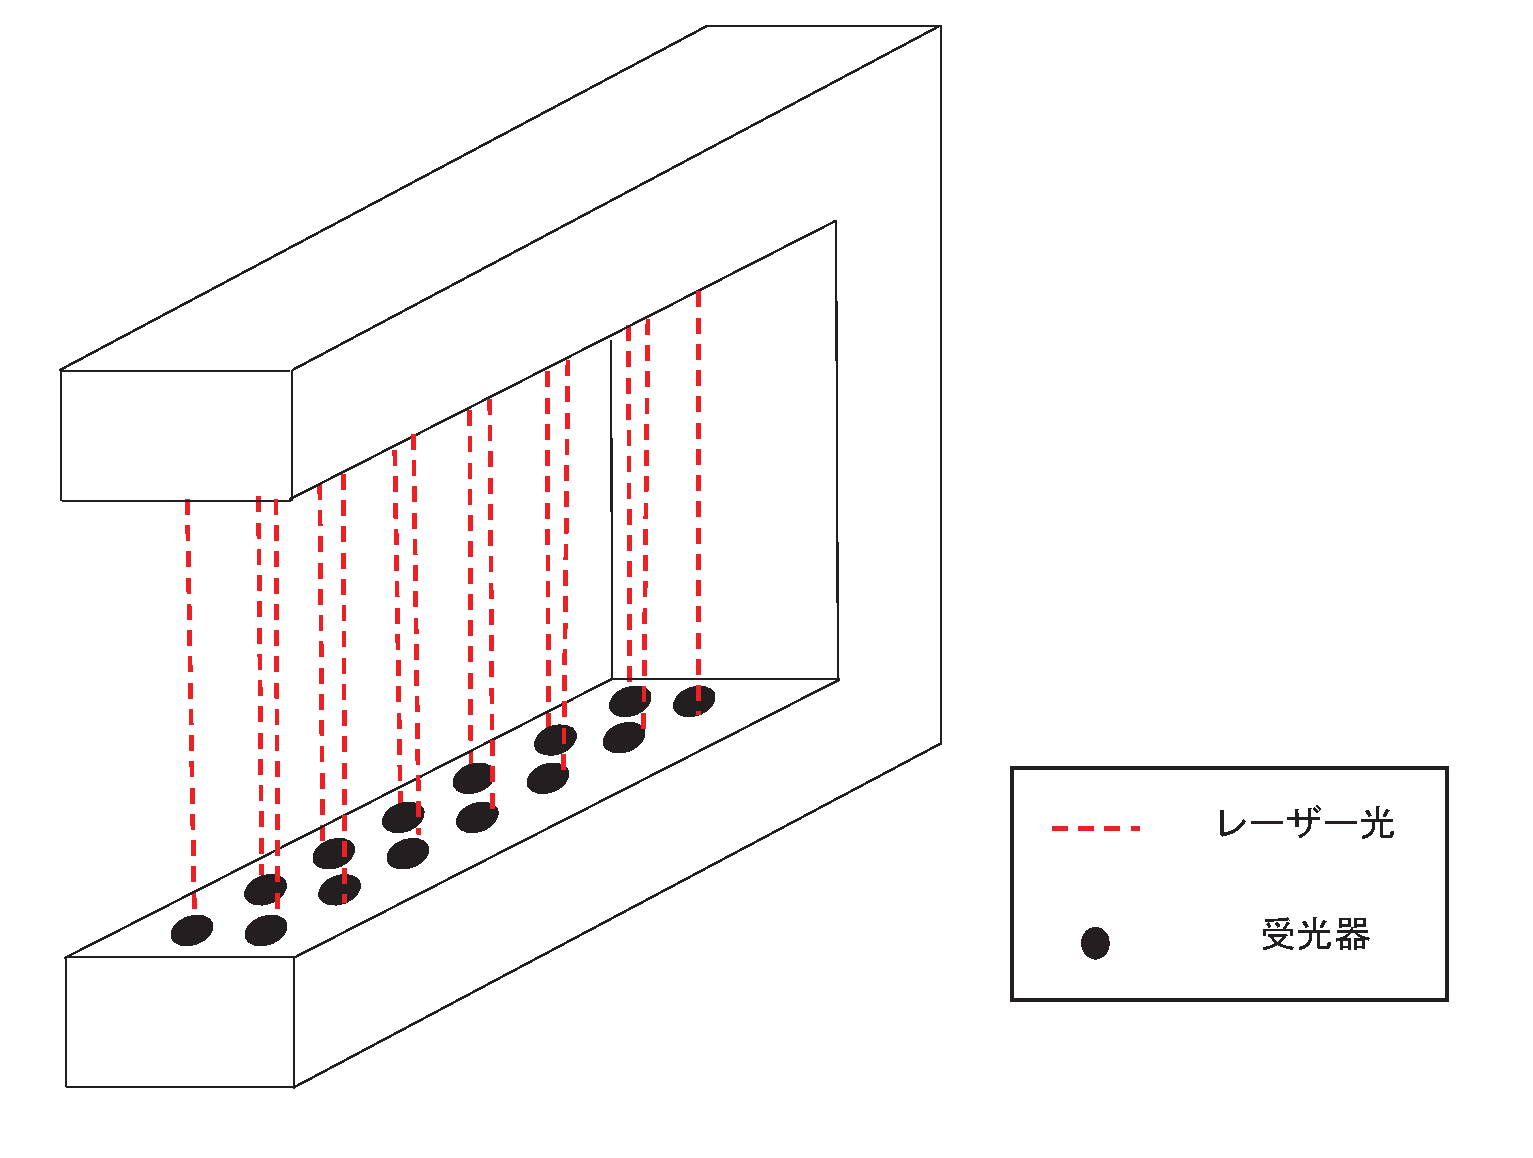
\includegraphics[width=10cm]{RazerDevice_image} \\

 \vspace{1mm}
  図3-1. レーザー光を用いたデバイスのイメージ
\end{center}

デバイスの上部に、計24個のレーザーを設置する。それと対になるように、下部に同数の受光器を設置する。この間を手が通過すると、レーザー光が遮られたことを受光器が検出する。実際に作成したデバイスを用いて、取得した手情報を画像に描画したものを、図3-2に示す。図3-3は使用したデバイスの写真である。

\begin{center}
  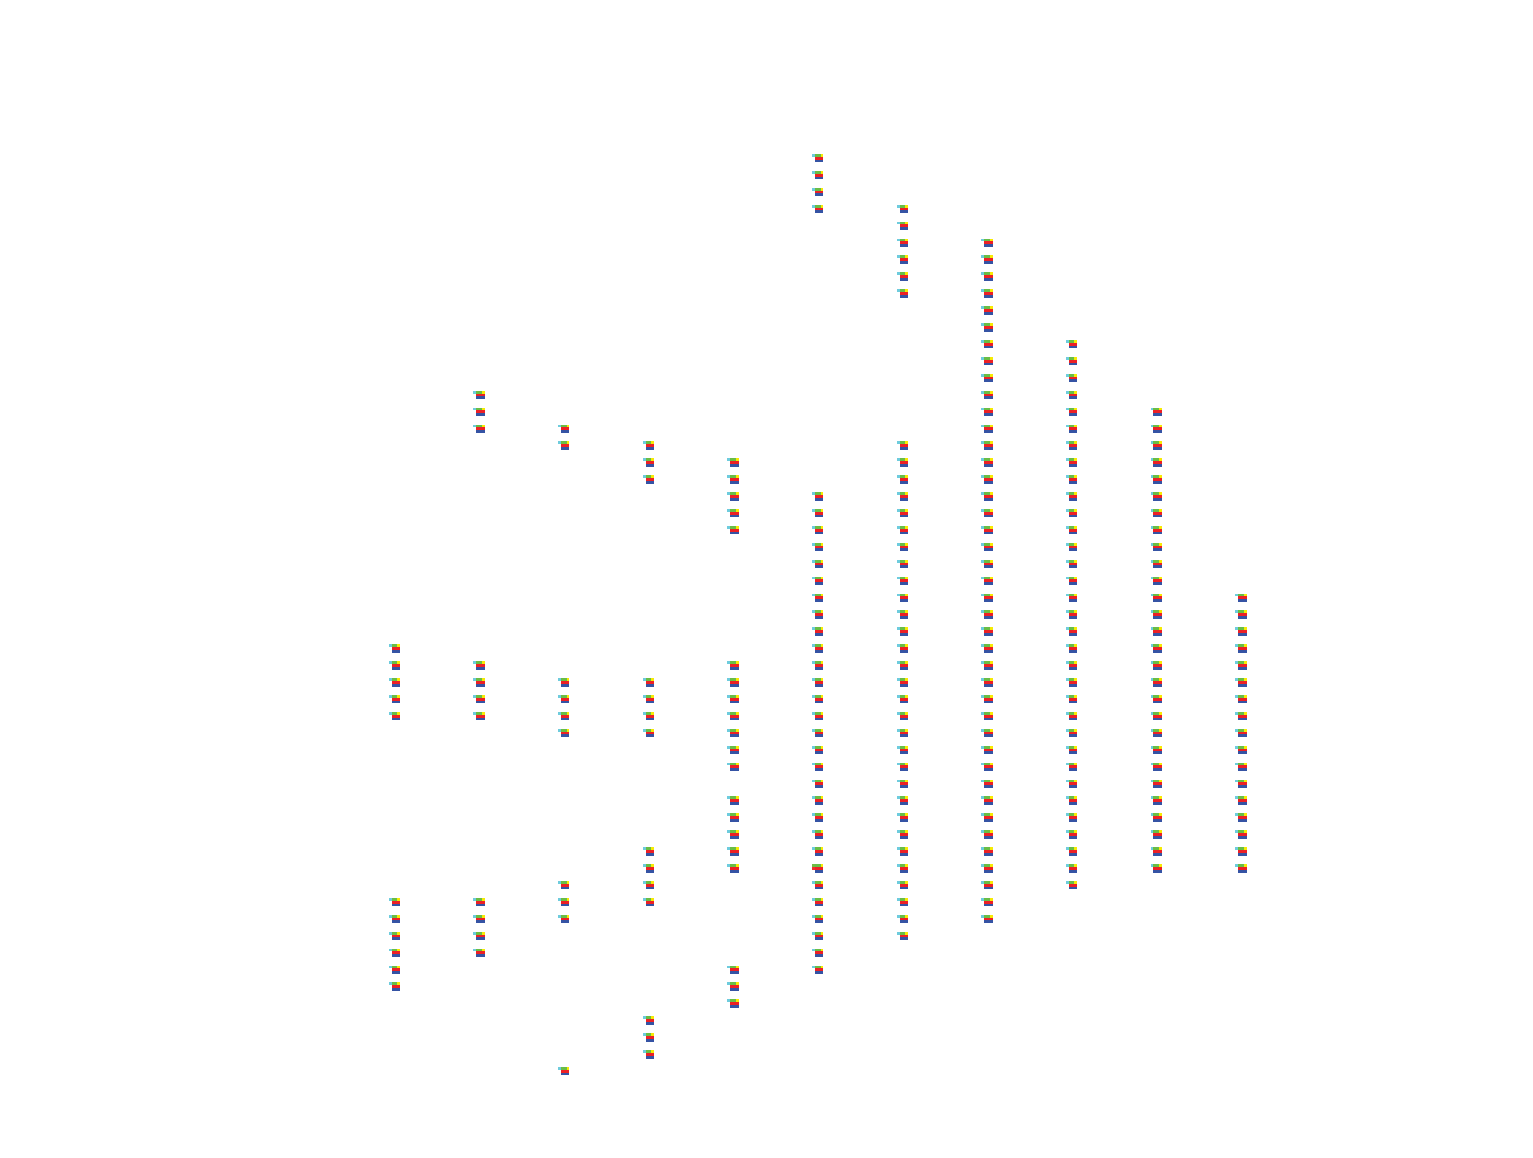
\includegraphics[width=10cm]{RazerDevice_getInfo.eps} \\

 \vspace{1mm}
  図3-2. レーザー光デバイスを用いて実際に得た情報
\end{center}

 \vspace{5mm}

\begin{center}
  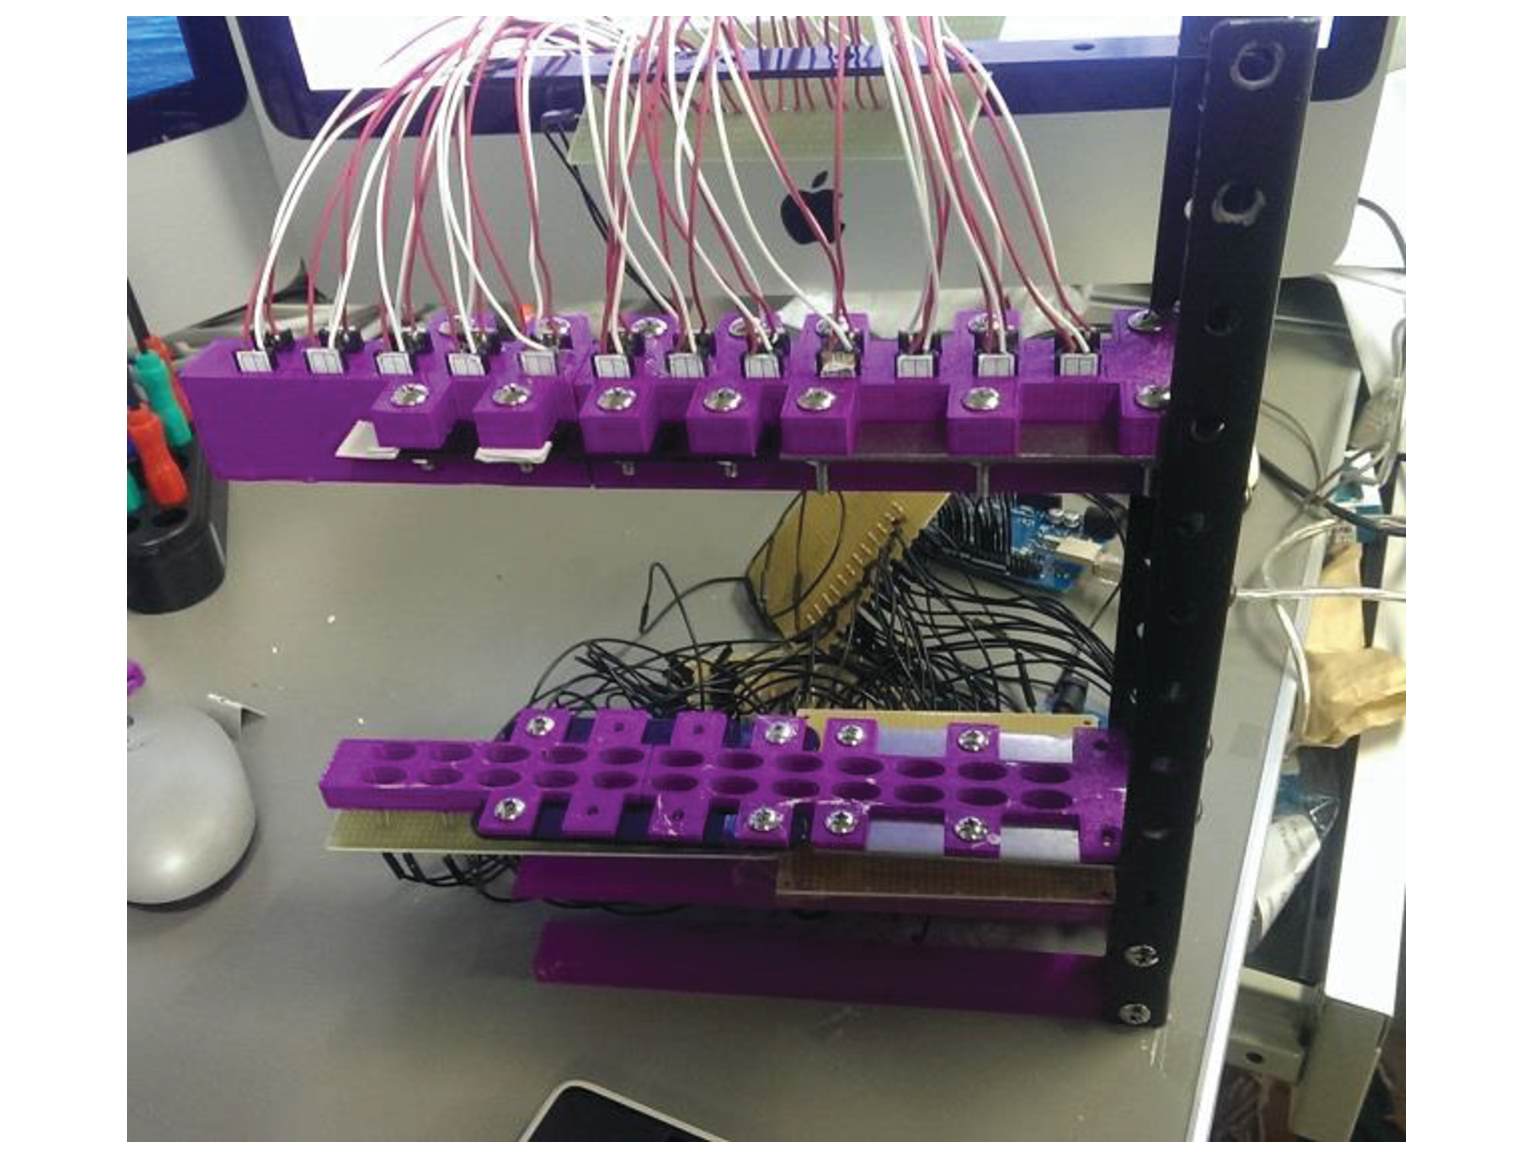
\includegraphics[width=10cm]{RazerDevice_real_color.eps} \\

 \vspace{1mm}
  図3-3. 実際に作成したレーザー光デバイス
\end{center}

図3-2より、レーザー光を用いた手の形状を認識が可能であることが伺える。しかしながら、このデバイスには問題が存在する。それは、レーザー数が足りないということである。手の情報を得るためには、スキャナーのように手を固定した形で通過させる必要がある。この制約は、動的な手情報を得ることができないことを示している。つまり、VRと組み合わせた直感的なハンドジェスチャーインターフェースを作ることは不可能である。だが、図3-2の結果から、認識したい物体の範囲より広くレーザーを設置することが出来れば、動的に手情報を得ることができると推測される。% このデバイスのイメージ用意してもいいかも
このことを踏まえて、レーザー光の代わりにWebカメラを用いたシミュレータデバイスを作成した。

% 3.2.2
\subsubsection{Webカメラを用いたシミュレータデバイス}
図3-4は、レーザー光の代わりにWebカメラを用いたシミュレータデバイスのイメージとなる。側面が一つ空いているボックスの上面と側面に対して、図3-4のようにWebカメラを設置する。レーザー光による検出を再現するために、Webカメラから得られた映像に対して、一定間隔毎に情報を取得する座標を設けることとする。カメラの対面に青いスクリーンを貼り付けることによって、間を青以外の物体が遮った時に、それを検出できるようにする。実際にボックスの中に手を入れて、取得した情報を図3-5に示す。図3-5は図3-4の上部に設置したWebカメラから取得した情報である。同様の手法で、横のWebカメラからも同時に情報を取得する。縦、横の二つの画像から手情報を三次元空間に構築して、同空間に生成したオブジェクトを動かすことにより、直感的なジェスチャーを可能にするための道筋を示す。図3-6は実際に作成したシミュレータデバイスである。

\begin{center}
  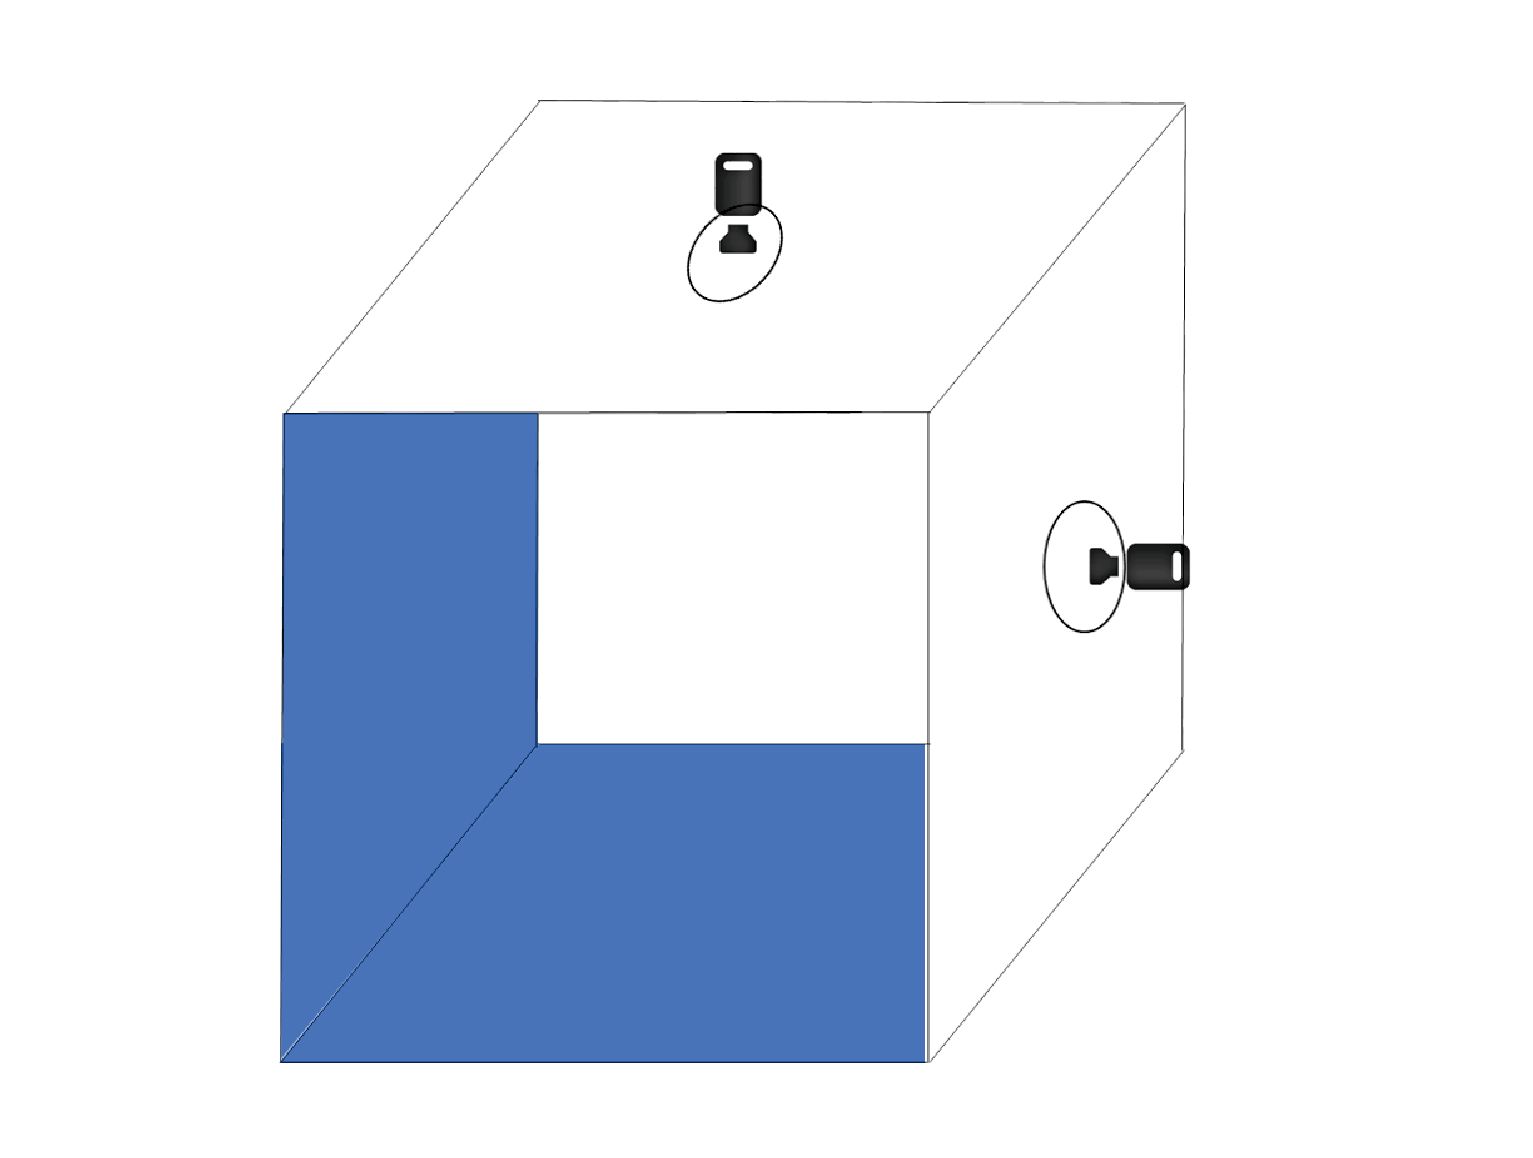
\includegraphics[width=10cm]{Simulator_image.eps} \\

 \vspace{1mm}
  図3-4. Webカメラを用いたシミュレータデバイスのイメージ
\end{center}

\begin{center}
  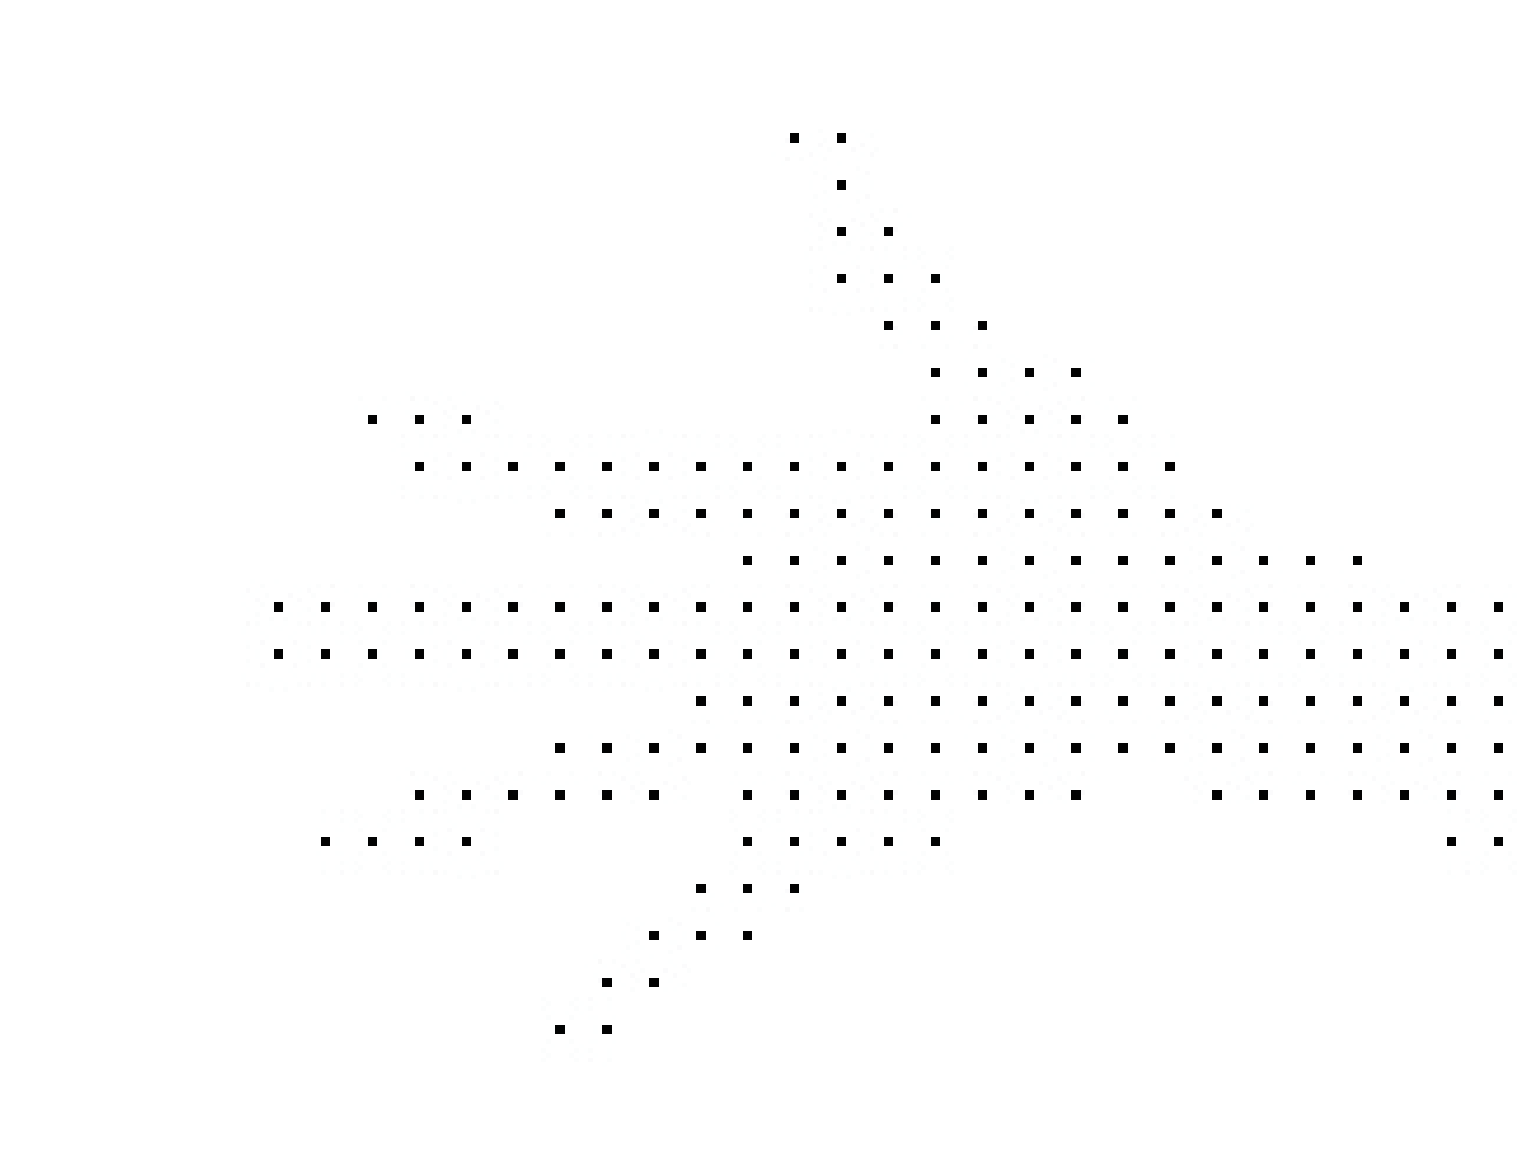
\includegraphics[width=10cm]{Simulator_getInfo.eps} \\

 \vspace{1mm}
  図3-5. シミュレータデバイスから得られた情報
\end{center}

 \vspace{10mm}
\begin{center}
  \includegraphics[width=10cm]{Simulator_real_color.eps} \\

 \vspace{1mm}
  図3-5. 実際に作成したシミュレータデバイス
\end{center}

% 3.2.3
\subsubsection{3Dオブジェクトと手情報の接触判定}
オブジェクトが存在する三次元空間に、正方格子点が存在すると考える。それらの点がオブジェクトの内部にあるのか、外部にあるのかを判定する。その判定結果と手情報を比較することによって、3Dオブジェクトを動かせるようにする。判定する方法について詳しく述べる。三次元空間を一定間隔の層に分ける。各階層毎に内部外部判定を行うことで、擬似的に三次元オブジェクトに対して内部外部判定を行うことができる。各階層毎の内部外部判定には、外積計算と Cauchy の積分定理を組み合わせた手法を用いる。ここで、外積計算による判定方法と、 Cauchy の積分定理による判定方法について説明を行う。一般的な特徴として、外積計算による方法は、くぼみや穴などを有するドーナッツ型の図形に対する内部外部判定が不利であり、かつ複雑形状の図形において、境界線から離れた内部で判定が困難である。Cauchy の積分定理による方法は、くぼみや穴などを有するドーナッツ型の図形に対する内部外部判定が有利である一方で、複雑形状の図形において、境界線付近での判定に難があるというデメリットが存在する。そこで本研究では、 Cauchy の積分定理の弱点を、外積計算による方法で補う手法を取る。






















